\begin{table}[h]
    \centering
    \caption[Threshold rules for labeling]{Rule-based thresholds used for multi-class labeling.}
    \label{tab:label-thresholds}
    \begin{tabular}{|c|l|}
    \hline
    \textbf{Label} & \textbf{Threshold Conditions} \\ \hline
    STOP & brake $>$ 0.5 AND throttle $<$ 0.2 \\ \hline
    RIGHT & steering $>$ 0.1 AND brake $<$ 0.5 \\ \hline
    LEFT & steering $<$ $-0.1$ AND brake $<$ 0.5 \\ \hline
    GO & throttle $>$ 0.5 AND $|\text{steering}|$ $<$ 0.1 \\ \hline
    \end{tabular}
\end{table}


\vspace{5em} 


\begin{figure}[h]
    \centering
    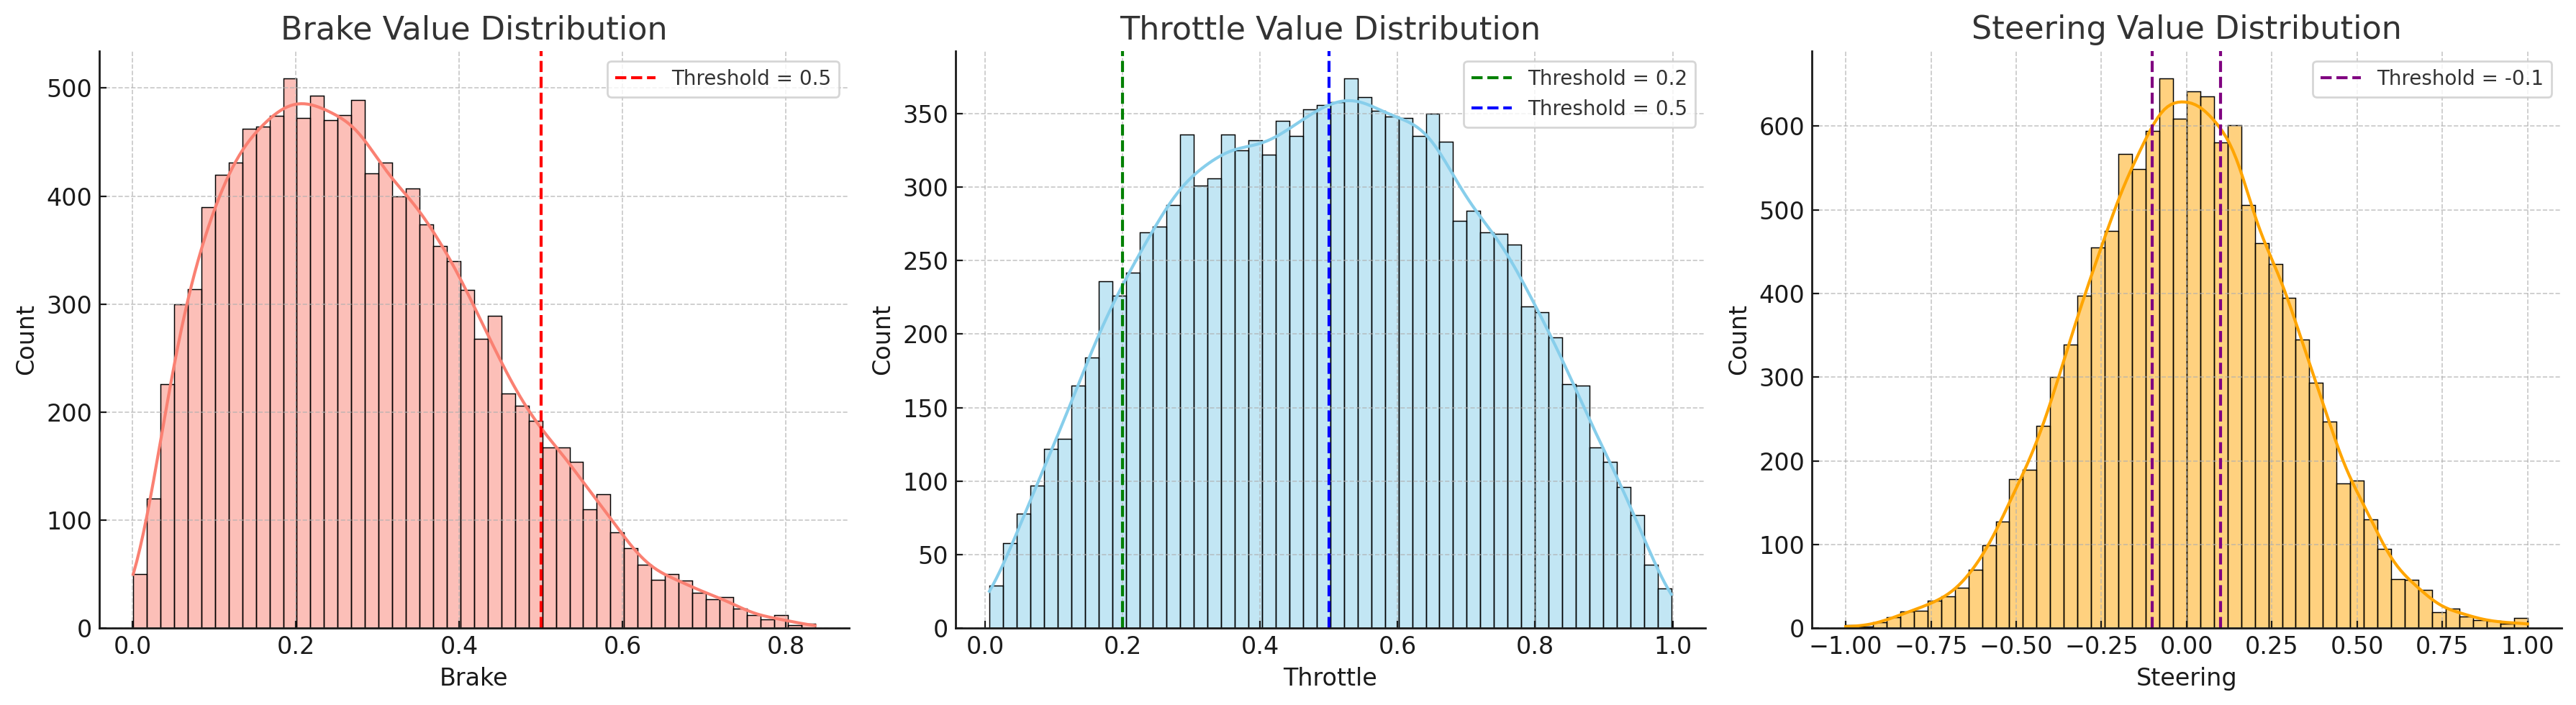
\includegraphics[width=\textwidth]{img/dataset/data_distribution_for_driving.png} 
    \caption[Control signal distributions for labeling]{Distribution of control signal values used for labeling. Vertical dashed lines indicate the empirically selected threshold values for brake, throttle, and steering.}
    \label{fig:threshold-histograms}
\end{figure}